\documentclass[12pt]{article}
\usepackage[top=2cm,bottom=1cm,left=2.5cm,right=4.5cm]{geometry}

\usepackage{parskip}
\usepackage{mathtools}
\usepackage{hyperref}
\usepackage{listings}
\usepackage{tikz}
\usepackage{csquotes}
\usepackage{rotating}
\usepackage[english]{babel}
\usepackage{booktabs,tabularx}
\newcommand{\ra}[1]{\renewcommand{\arraystretch}{#1}}
\usepackage[acronym,nonumberlist,toc]{glossaries}
\usepackage{url}
\usepackage[utf8]{inputenc}

\usepackage[
    backend=biber,
    natbib=true,
    url=true,
    style=apa,
    maxbibnames=99,
    date=short,
uniquename=init]{biblatex}
\DeclareLanguageMapping{english}{english-apa}
\linespread{1.3}
\def\layersep{5cm}
\def\outputlayer{10cm}
\input{commands}
\input{acronyms}

\makeglossaries
\addbibresource{risk.bib}
\begin{document}
\input{titlepage}
\clearpage
\input{disclaimer}
\clearpage
\input{acknowledgements}
\clearpage
\input{abstract}
\clearpage
\tableofcontents
\clearpage
\listoffigures
\clearpage
\listoftables
\clearpage
\printglossaries
\clearpage

\section{Introduction}
\label{sec:Introduction}

A recurring observable trend nowadays, is the active participation of single consumers in the financial markets~\citep{barasinska}. As such new structures to support this have been created in the banking sector. Banks offer their consumers stocks, portfolios and various other financial products, tailored to an individuals needs. 

This approach though can be often lacking as individual preferences are not always accounted for, and most of the time standard questionnaires are used to classify customers in specific segments.

One metric that could be used in this case and would offer a little more information when creating suggestions for financial products tailored to the individual needs of a customer, is \emph{the willingness to take risk} that each individual presents. 

As the risk of stocks and portfolio options can be calculated based on the expected returns, among other data, one could use this metric to asses which financial product would be appropriate for an individual, based on his risk-profile.

Various researchers such as~\citet{individualRiskAttitudes} have proposed a variety of determinants, and attributes which would express a certain level of risk-willingness or averseness in individuals. 

Although such metrics do not display causal relationships, but merely correlations, they could be used in conjunction with data-exploration algorithms such as machine-learning to recognize common patterns between customers that display similar determinants.

Calculating financial risk though is a very complicated manner. By recognizing that this problem could easily be solved for an individual case, one might think of it as a problem of classifying individuals in certain risk-category groups. 

The ability to provide classification from a variety of metrics, for a large number of data sets is a main feature exhibited by artificial neural networks. 

To achieve classifiable information, the questionnaire should, in the end, provide a metric that would reflect the willingness to take risk for an individual customer. 

This metric should be able to classify individuals in certain risk-classes which would then allow, for example a bank-representative, to make more concrete suggestions on the products offered to the customer. This could then be used in a neural network to automate the classification process of individual cases.

For this reason, the project described in this paper will try to solve following problem:

\textit{Which metrics and how should those metrics be evaluated when using neural networks in order to associate individual willingness to take risk with a specific risk class.}

\section{Theoretical Background}
\label{sec:theoretical_background}

This section will provide a brief introduction into the main theoretical premises utilized in implementing this project. It is structured in the following way:

\begin{enumerate}
    \item The first subsection will provide an introduction into the definition of financial risk, and its scope in this paper.
    \item The second subsection will introduce neural networks and their functions.
    \item Subsequently the application between the two will be explained.
\end{enumerate}

After reading this Section, the reader will be able to grasp some of the technical aspects discussed in this paper, as well as some concepts related to machine learning and data sciences.

\subsection{Financial Risk}
\label{sub:financial_risk}

The measurement and control of risk is a major topic even today~\citep{finRisk}.~\citet{finRisk} states that financial risk is associated with the statistical uncertainty of the final outcome, and is measured by its volatility. 

Humans will take financial risk at different levels, in order to arrive at financial gains. Some will test highly risky affairs which yield higher rewards, while others will prefer less risk at the downside of smaller returns on their financial investment.

\citet{financialRiskTolerance.pdf}, defines such a metric as the \emph{financial risk tolerance} which is stated to be the amount of uncertainty an individual is able to accept when making a financial decision.

\citet{financialRiskTolerance.pdf}, ascertains through the various literary research that the task of defining metrics in order to conclude on an individuals risk tolerance is quite hard, although a variety of research concludes on the correlation of a number of factors such as gender and education. This topic will be revisited at a later stage in this paper as part of Section~\ref{sub:determinants_risks}.

In the case of this paper, financial risk will be defined as the risk taken by an individual when he chooses to invests in a stock option, a portfolio or bond options with the ultimate goal of expanding his monetary gain. The financial risk taken therefore, is the loss of the investment in case of risk materialisation~\citep{finRisk}. 

This paper will not consider financial risk per se in the classical sense, which would mean determining the downsides of a particular investment, rather it will consider itself with the risk category an individual is classified in based on his determinants chosen as part of the literary analysis in Section~\ref{sub:determinants_risks}

\subsection{Machine Learning}
\label{sub:neural_networks}

Neural networks and deep learning are in essence machine learning algorithms, where in this case deep learning is a more specific form of machine learning~\citep{deeplearningbook}. For the purpose of this paper, the definition presented below is derived from~\citet{deeplearningbook}. 

The formal definition of the learning process of an algorithm is defined as: 
 
`A computer program is said to learn from experience \textit{E} with respect to some class of tasks \textit{T} and performance measure \textit{P}, if its performance at task in \textit{T}, as measured by \textit{P}, improves with experience \textit{E}.`\footnote{\citet{mitchel97} p.3}. 

The task \textit{T}, is more accurately a task, that is difficult to solve with a fixed, traditional program. The task should also not be confused with the process of learning, since the task itself is the problem that needs to be solved.

\subsubsection{The Task \textit{T}}
\label{subsub:task}

As iterated before, machine learning itself is a tool that allows a researcher to solve a certain task, a problem. 

The problem to be solved is deemed to be too difficult to be solved by a traditional fixed program designed by a human being. Often people mistake the task itself with the process of learning, that is not the case. 

The task is the problem at hand, the learning process is the way in which the program can attain its ability, as for example a trainee who needs to learn from experience, to solve the task at hand~\citep{deeplearningbook}.

A machine learning task is usually described in terms of how the machine learning system should process a certain example. 

The example itself is a collection of features which has been measured quantitatively through an experiment and is presented as a dataset that the machine learning algorithm should process. 

The features themselves are described as $\textbf{x} \in R^n$ where each entry $x_i$ represents one feature out of all the recorded features. The types of task, which define the type of network that needs to be used, are briefly described in Section~\ref{subsub:task_types}. 

\subsubsection{Task Types}
\label{subsub:task_types}

The learning activity is based on how a machine learning algorithm will process an \textbf{example}. The example is composed of a collection of \textbf{features}, and consists of a vector $x \in R^n$, where each $x_i$ of the vector is just another feature of the example. 

An example of such a feature are the values of the individual pixels in an image, if the task is image recognition. Some of the more common tasks that can be solved by machine learning are as follows:

\begin{itemize}
    \item Classification: The task here is to specify in what category \textit{k} a certain input belongs to. These type of algorithms are used for example for classifying images to objects. A function $f(x)$is computed based on the data learned. $f(x)$ is then a function that can specify in which category \textit{k} subsequent inputs belong to.
    \item Regression: The task here is to predict a numerical value given some input. The function $f(x)$ that is calculated is similar to the one of the classification algorithm with the exception that the output is a numerical value. A simple example of this is the prediction of the claim amount an insured individual will make, or the future price of securities.
    \item Transcription: The task in this instance, is to observe an unstructured representation of some kind of data, and try to transcribe it in textual form.
    \item Machine translation: In this task the computer tries to translate one language to another. The most common application is the translation of two natural languages e.g. English to French. 
    \item Structured output: Any tasks, where the output is a vector, that contains important relationships between the different elements. An example would be parsing of natural languages in trees that describe grammatical structures.
    \item Anomaly detection: The program will flag data that is not conforming to the usually observed data as an anomaly. Usage is e.g. Credit card fraud, or in anti-virus software.
    \item Synthesis and sampling: The task is to generate new examples, based on the already existing data. This is interesting as for example the program might be tasked to create a movie script, or create large volumes of music.
    \item Imputation of missing values: The task is to be able to predict missing values in datasets
    \item Denoising: A corrupted example is given which was corrupted by an unknown process, and the program hast to predict a clean example through another clean example x.
    \item Density estimation or probability mass function estimation: Advanced use-case where the machine learns a probability density function. An example would be the distribution of a disease among a large population, in order to identify common problem sectors.
\end{itemize}

\subsubsection{Performance Measure \textit{P}}
\label{subsub:performance_measure}

The performance measure evaluates, quantitatively, how good the network performs for a specific task. As an example consider the case of a classification task, the performance measure would be the accuracy of the network in predicting the correct class~\citep{deeplearningbook}. 

Usually the performance is measured based on either the \textbf{accuracy}, that means the amount of correctly identified examples or the \textbf{error rate}, which designates the proportion of all the examples where the algorithm produces an incorrect output~\citep{deeplearningbook}.

To evaluate the performance measures after reaching a satisfying error rate or accuracy, the performance is measured again based on a \textbf{test-set} of data that the network never saw before. 

These performance metrics though are not universal, and thus although it may seem straightforward to define them, it is not.

The decision on how to define them is often decided how fine-grained the error metric should be, as an example for this the transcription task, in which the choice often is between successfully transcribing a whole sentence, or the individual words~\citep{deeplearningbook}. 

In addition, it is often not clear what should account as an error metric, as in the case of a density estimation, where the algorithm does not try to guess an output.

All these considerations, are part of the design phase of the network and are always depended on the type of task the network should perform~\citep{deeplearningbook}.

\subsubsection{The Experience, \textit{E}}
\label{subsub:the_experience}

Machine learning algorithms, as partly referenced in Section~\ref{subsub:task_types}, can be split in either \textbf{supervised} or \textbf{unsupervised} learning algorithms. 

The experience the algorithm processes can be defined as the \textbf{dataset} which is chosen as an input for the machine learning algorithm. The \textbf{dataset}, are the results of quantitatively measured experiment, and each identifier is considered to be a feature $x_i$.

In an \textbf{unsupervised} learning algorithm, the algorithm experiences the whole dataset and tries to extract useful properties out of it without requiring explicit labeling by a user, for example a denoising network, or a k-means algorithm. 

The machine learning algorithm in unsupervised learning tries to guess the probability distribution of $y$ or other types of distributions that can be \emph{learned} by viewing a set of examples $x_i$ contained in a dataset $\vec{X}$.

In a \textbf{supervised} learning algorithm, the algorithm experiences the dataset which is associated to a specific \textbf{label} or \textbf{target}. 

This is approach is generally used as part of classification algorithms, such as when classifying plants based on the features of their iris. 

Generally speaking a supervised learning algorithm tries to, by observing a dataset $x$, predict the probability of it being $y$, so algorithmically guesses $p(y|x)$. 

The term supervised derives from the fact that the user of the network provides the network with a set of labels, like an instructor in school where he provides exercises to the pupils and subsequently teaches them how to solve them, through those examples.

In contrast, in an unsupervised training task, the algorithm tries to make sense from the data all by itself with no input from an instructor. 

The terms themselves have not been formally defined by researchers, and the scientific community has not reached a definite clear distinction between the two~\citep{deeplearningbook}, this topic however is not in the scope of this paper.

Machine algorithms experience a certain dataset. The dataset can be usually thought of as a matrix where each row is one example of \textit{n} features. 

In supervised learning algorithms, the last column(s) of the matrix is usually reserved for for the \textbf{label}. The label is not always a single number, but can often take the form of a vector, for example a binary coded vector.

\subsubsection{Overfitting, underfitting and capacity}
\label{subsub:overfitting}

One of the most important and challenging aspects in machine learning is the concept of \textbf{over-} and \textbf{underfitting}. 

\textbf{Overfitting} generally means that due to outliers in the underlying dataset, the model generated by the machine learning algorithm displays a large gap between the error produced by the training and the testing set.

In the case of \textbf{underfitting}, the outliers in the underlying dataset have the effect that the machine learning algorithm cannot attain a low enough error value.

Over- and underfitting, can be controlled through an attribute called \textbf{capacity}. Capacity generally expresses a wide variety of functions, which will not be explained here. 

One example for such a function although, would be to standardize the input data, in order to make the data more homogeneous, and reduce big outliers in the input. 

Such an approach is discussed in Section~\ref{subsub:norm_stand_one_hot}.

\subsubsection{Normalization, Standardization and One-hot-encodings}
\label{subsub:norm_stand_one_hot}

Normalization is not connected with neural networks and machine learning as a concept, yet it is connected to the datasets the algorithms have to process. In statistics normalization can have a variety of meanings. 

The simplest case of normalization is the normalization of ratings, in which different rating measures are converted into a common scale. 

There is also, the case of score normalization in statistics, in which different probability distributions are aligned onto a normal distribution~\citep{normal}.

In the case of this paper, normalization stands for the creation of shifted and scaled versions of statistics, where the intention is that these \textbf{normalized values} eliminate anomalies and big outliers in the dataset. 

Normalization can be used as a technique to avoid overfitting or underfitting data, and is expressed through following formula:

\begin{equation}
x_{new} = (x - x_min)/(x_max - x_min)
\end{equation}

Standardization refers to the conversion of data, in such way that the data is transformed to have zero mean and unit variance. This is described by following formula:

\begin{equation}
x_{new} = (x - \mu) / \sigma
\end{equation}

One-hot-encoding stems from digital circuits, and is employed in data-sciences when encoding categorical variables to values. 

Formally, when encoding categorical data one could use a values between \textit{1..n}, where \textit{n} amounts to the distinct elements in the categorical data. Usually though, it is not desired to have ordinal characteristics into a dataset that does not have any order. 

An example for this would be the case of a gender, with values \textit{male} and \textit{female}, where if the value \textit{male} would be mapped to a 1 and \textit{female} to 0 it could imply that $male\ge{female}$~\citep{one_hot}.

For this purpose, one-hot-encoding transforms these categorical data into binary encoded vectors, more formally, a single variable with \textit{n} observations and \textit{d} distinct values gets converted to a \textit{d} binary variable with \textit{n} observations each. 

Thus in the previous example, the values \textit{male} and \textit{female}, would be become (1,0) if the observation was male and (0,1) if the observation was female.

\subsubsection{Deep Neural Networks}
\label{subsub:deep_nets}

The main form of deep learning used in this paper is the so called deep feedforward network, also called multilayer perceptron. The multilayer perceptron constitutes the quintessential model for deep learning networks. 

The goal of a network is the approximation of some function $f*$. The algorithms are called feedforward since data flows from the inputs towards the outputs, and no feedback connections exist between the different layers. 

An alternate form of it would be a network which feeds the information it gets from the computations back to itself at every step of the iteration. Such a network is called a recurrent neural network.

The reason these algorithms are called networks, is that they are a composition between different functions which execute in a chain depending on the input. 

Backpropagation is a technique employed in order to feed the prediction error described in Section~\ref{subsub:performance_measure} back into the weights of the network. 

The name deep stems from the fact, that due to having more than 2 functions there is a certain depth to the network, in other words the intermediate hidden layers provide this depth.

The algorithm used in the multilayer perceptron is expressed by the following function~\citep{theanoTutorial}:

$f: R^D \rightarrow R^L$, where $D$ is the size of input vector $x$ and $L$ the size of the output vector $f(x)$. $f(x)$ is expressed as~\citep{theanoTutorial}:

\begin{equation}
    f(x) = G(b^{(2)} + W^{(2)}(s(b^{(1)}+W^{(1)}x)))
\end{equation}

With $b^{(1)}$,$b^{(2)}$ being the bias vectors and $W^{(1)}$,$W^{(2)}$ being the weight matrices. $G$ and $s$ are activation function. A typical choice for $s$ are either $tanh$ or $sigmoid$.

The output of the neural network is achieved by $o(x) = G(b^{(2)} + W{(2)}h(x))$. 

$G$ is usually a $softmax$ function in the case of classification problems. In the case of the network being portrayed here, the function used is logistic regression~\citep{theanoTutorial}.

The optimization problem, in the case of this paper is solved through \emph{stochastic gradient descent}~\citep{theanoTutorial}, which has the formula:

\begin{equation}
    Q(w) = 1/n\sum_{i=1}^{n}Qi(w)
\end{equation}

\subsubsection{Support Vector Machine}
\label{subsub:svm}
%TODO: https://www.ncbi.nlm.nih.gov/pmc/articles/PMC3288439/
A \gls{svm} is a widely employed machine learning classifier algorithm. It has been often proven to work more efficiently than neural networks in certain classification tasks such as binary classification~\citep{up, 04443437.pdf}. 

They were invented by~\citet{svm.pdf}, with the purpose of pattern recognition in a binary-classification system.

The basic idea behind it is that the input vectors are non-linearly mapped to a very high-dimension feature space, where a linear decision surface is to be constructed. 

An SVM is quite similar to feedworward networks, yet different enough to be a standalone machine learning algorithm. 

A support vector machine operates on the following principle~\citep{dlsvm}:

Given training data $(x_n,y_n)$, $n=1,\ldots,N$, $x_n \in R^D$, $t_n \in {-1,1}$, the algorithm that a SVM employees to process the dataset is as follows~\citep{dlsvm}:

\begin{equation}
    \min1/2w^Tw + C\sum_{n=1}^{N}{\xi_n}
\end{equation}

\begin{equation}
    s.t.\ w^Tx_nt_n \geq 1-\xi_n, \forall n
\end{equation}

\begin{equation}
    \xi_n \geq 0, \forall n
\end{equation}

$\xi_n$ are so called slack variables, and are added to the algorithm in order to transform an inequality to an equality when dealing with optimization problems. The optimization equation for the SVM is also called L2-SVM and minimizes the squared hinge loss~\citep{dlsvm}:

\begin{equation}
   \min_{w} 1/2w^Tw+C\sum_{n=1}^{N}\max(1-w^Tx_nt_n,0)^2
\end{equation}

Finally, to make the prediction the SVM employees an $\arg \max_{t}(w^Tx)t$. An $\arg \max$ selects the maximum points of a function, in this case the class which displays the maximum probability.

\section{Literature Review}
\label{sec:literature_review}

This section will be reviewing available literature that focuses on creating neural networks to asses risk in different settings. 

Some of the literature reviewed here does not directly apply to the case at hand, yet yields useful information in what kind of methodology that should be applied in order to create the implementation detailed in Section~\ref{sec:methodology}.

\subsection{Determinants of Risk}
\label{sub:determinants_risks}
%TODO: Add another paper from our big collection!

\citet{dp4807.pdf} researches the question if it is at all possible to investigate individual risk attitudes using a survey. \citet{dp4807.pdf}, try to asses the viability of using a hypothetical lottery, and risk self-assessment when measuring risk-attitudes of individuals. 

Their research is based on~\citet{individualRiskAttitudes}, and therefore their questions are modelled in a similar fashion. 

Their findings indicate that hypothetical lotteries and self-scaling questions are generally good indicators to measure someones risk attitude. 

\citet{dp4807.pdf} though, argue that the heterogeneity of the results point out that it might be better to use more context specific questions based on the problem at hand. 

The results of this study influenced the decisions taken in Section~\ref{sec:methodology} while creating the survey for this paper.

A wide array of research exists in the social, financial and economical studies on the determinants of risk in individuals and in groupings. For the purpose of this paper, a number of those which address financial risk directly were chosen.

\citet{individualRiskAttitudes} states that their am was to examine risk attitudes based on a large representative survey provided by \gls{soep}\@. 

The study was then complemented by a smaller field study which examined the general willingness of an individual to take risk, based on the findings of the previous examination. 

\citet{individualRiskAttitudes} then proceeds to expand their findings in order to correlate the general risk with more specific risk types such as smoking, financial risk and etc. 

In the findings the group concludes that gender, age, height and the parental background do indeed correlate with risk attitude an individual displays. 

In addition to these determinants, choices such as investment in stocks and doing sports have been found to contribute to the willingness of an individual to take risk.

\citet{individualRiskAttitudes} used a financial lottery in order to verify these results in the field experiment, this approach will be used by this paper in Section~\ref{sec:methodology}.


\subsection{Financial risk with Neural Networks}
\label{sub:financial_risk_nn}

Finance is always a subject in statistics, and as such a large number of literature exists which employees neural networks in financial contexts. 

In the following this papers will concentrate itself with literature that is more akin to the problem being investigated, and describe tasks which are classification or regression tasks.

\citet{instanbulStock} investigates the application of neural networks in the Istanbul stock market, and developed an artificial neural network in order to perform a time-series prediction. 

The application implemented consisted of a simple multilayered perceptron, which consisted of 1 input layer, 1 hidden layer and an output layer. 

The input layer consisted of 10 technical features used in time-series predictions of stock. The output consisted of predicting the movement of the Istanbul stock exchange.

%TODO: Add the citation for regression vs classification.
The results obtained by the \gls{ann} were then compared with the results that were obtained by the \emph{SVM} which used similar feature metrics as input. 

The conclusion the researchers reached was that both methods help obtain a significant performance in predicting the movement of the stock exchange, yet the average performance of the \emph{ANN} was higher than the one produced by the \emph{SVM}. 

This coincides with the experience of other researchers~\citep{equivalence,caruana.icml06.pdf}, which showed that \emph{ANN} are far better at predicting time series, or basically regression data as are \emph{SVMs}, yet SVMs should excel at classification tasks, as this is their background.

Building on that research,~\citet{bitcoinNN} try to predict the evolution of bitcoin price as a time series. 

The authors opted for a simple neural network using Theano, and deciding to not to asses price-to-price predictions but rather, train the network depending on the trends bitcoin prices show at between a certain time period, namely: \textit{up,margin and down}. 

Their implementation uses the predictions made by the network in order to decide on trading the bitcoins.~\citet{bitcoinNN} implement following strategy when the program chooses to trade: 

In the case of \textit{up} they always trade, in \textit{margin} they do nothing and in \textit{down} there is the option to short-sell the available volume. 

Their results were quite interesting, as the network correctly predicts, after a certain amount of time the trends in the price of bitcoin, and thus also traded quite successfully, or so it seemed.

Yet \citet{bitcoinNN}, state in their results, that the predictions made by the network, seemed to good to be really true, since when compared to more advanced on-line learning algorithms, their simple network was outperforming the rest. 

The end result showed that the network itself did not really outperform and that the baseline profit was close to zero. The reason for the misinterpreted results, was due to the way the time-series data was formatted and fed into the performance evaluation function. 

The important takeaway from the research, is that due to the complexity of stock markets, and in general the data available the underlying data should always be carefully prepared before using it as an input into the neural network. 

A careful review of the end result is also needed in order to ensure that the networks predictions are actually valid with respect to over- and underfitting.

\citet{04443437.pdf} discussed risk evaluation of project financing. Project financing is a way is a way to finance large scale public projects, and stems from Private Public Partnerships, and the metric assessed by the authors is the overall risk posed by an entity when investing in such an endeavour. 

The authors use a total of 18 features, with one output value which describes the risk score computed by experts. The results are stated by the authors to be satisfactory, yet one of the problems with the training results, and in general was the low availability of input data. 

This research though, shows that neural networks can be used in complex settings to asses risk, in which the features used are non-exhaustive.

It can be thus concluded that neural networks are actively being used in finance to account for a variety of subjects, often those subjects consider themselves with regression tasks, yet there are also instances in which classification problems are analyzed. 

Furthermore the application of neural networks has not been fully realized at present, with most classification systems using pure machine learning algorithms. The following section will investigate the usage of neural networks in various settings that relate with risk-classification.

\subsection{Various risk with \gls{nn}}
\label{sub:various_risk_nn}
%TODO: Add another paper

\citet{riskAssesmentInternalAuditing} starts of with introducing the subject of risk assessment, applied to internal auditing, where risk assessment usually is based on pattern recognition, due to the fact that an unexpected deviation is symptomatic of risk. 

It's application in internal auditing risk assessment can help auditors understand the underlying data that leads to an assessment. 

The example used by~\citet{riskAssesmentInternalAuditing}, is that as an expert, only continuous exposure and experience can yield good results. If a network is exposed to the assessment of the experts, it will in the end figure out the combination of variables used by the expert in order to make his underlying assessment. 

Of interest is that the author compared the results taken by the neural network, and traditionally used statistical models. The author concluded that the neural network had made a positive impact and thus was more accurate than the statistical models.

\citet{14_1_3.pdf} tries to construct a neural network in order to asses the credit risk posed by clients at banks, when applying for a loan. The authors compared neural networks with the discriminant analysis performed usually by the banks. 

The results state that the neural networks do add value in terms of the correctly classified samples, by a margin of around 8\%.~\citet{14_1_3.pdf} state that although the network performed better, discriminant analysis should be used with neural networks, as discriminant analysis allows for an easier identification of the key variables that influence the end-result of the metric.

What can be seen in this section is that neural networks are a viable tool in predicting risk, and in general risk assessment of either sentiment, or concrete values. 

If the key features that actually influence the network are identified before usage of the network, the performance could be significantly better than traditional methods. 

Artificial neural networks can also be seen as a valid complement to existing alternatives, where as pointed out by~\citep{14_1_3.pdf}, there are scenarios where a combination of techniques would yield better results.

\citet{JILSA20111} builds on the theoretical standpoint of using \emph{ANN} for credit risk management/prediction in the case of Italian manufacturing companies. To achieve this the researchers build a multilayer perceptron network, using the common standard backpropagation algorithm to train the network, the findings were to be compared with similar research performed by \citep{anathema}. 

The results of this experiment revealed that neural networks are a good tool in order to reveal complex relationships between the input data, for example insights can be gained by looking at the individual weights assigned to each input in order to asses the importance of a certain input metric.

\cite{JILSA20111} state, that although no clear statement can be made about which approach is better in the case of statistical vs dynamic algorithms for credit risk analysis, \emph{ANNs} are deemed to be viable and due to the fact that more and more processing power is available, they will continue to grow as research tools in this domain.

\section{Methodology}
\label{sec:methodology}
\begin{figure}[ht]
    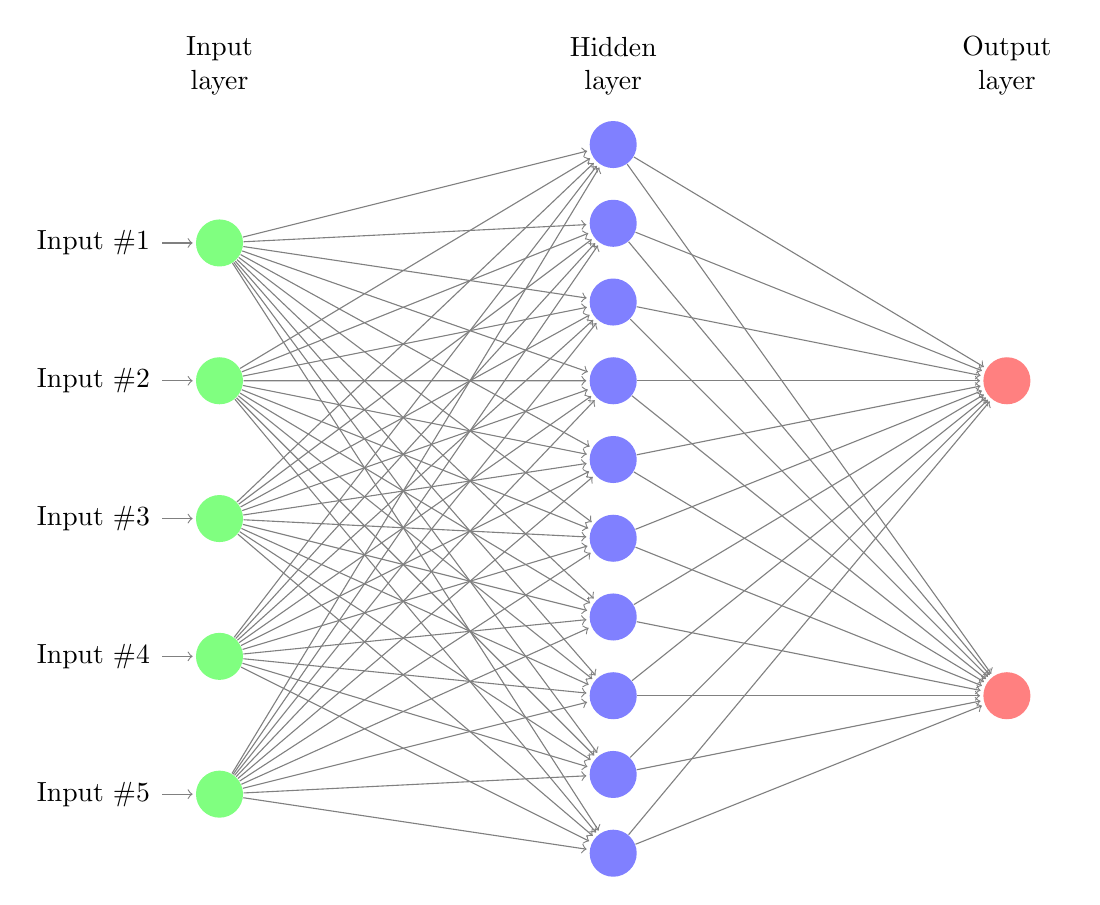
\begin{tikzpicture}[shorten >=1pt,->,draw=black!50, node distance=\layersep]
        \tikzstyle{every pin edge}=[<-,shorten <=1pt]
        \tikzstyle{neuron}=[circle,fill=black!25,minimum size=17pt,inner sep=0pt]
        \tikzstyle{input neuron}=[neuron, fill=green!50];
        \tikzstyle{output neuron}=[neuron, fill=red!50];
        \tikzstyle{hidden neuron}=[neuron, fill=blue!50];
        \tikzstyle{annot} = [text width=4em, text centered]

        % Draw the input layer nodes
        \foreach \name / \y in {1,...,5}
        % This is the same as writing \foreach \name / \y in {1/1,2/2,3/3,4/4}
        \node[input neuron, pin=left:Input \#\y] (I-\name) at (0,-\y*1.75 cm) {};

        % Draw the hidden layer nodes
        \foreach \name / \y in {1,...,10}
        \path[yshift=0.5cm]
            node[hidden neuron] (H-\name) at (\layersep,-\y cm) {};

        % Draw the output layer node
        \foreach \name / \y in {1,...,2}
        \path[yshift=0.5cm]
            node[output neuron] (O-\name) at (\outputlayer,-\y*4 cm) {};;

        % Connect every node in the input layer with every node in the
        % hidden layer.
        \foreach \source in {1,...,5}
        \foreach \dest in {1,...,10}
        \path (I-\source) edge (H-\dest);

        % Connect every node in the hidden layer with the output layer
        \foreach \source in {1,...,10}
        \foreach \dest in {1,...,2}
        \path (H-\source) edge (O-\dest);

        % Annotate the layers
        \node[annot,above of=H-1, node distance=1cm] (hl) {Hidden layer};
        \node[annot,left of=hl] {Input layer};
        \node[annot,right of=hl] {Output layer};
    \end{tikzpicture} 
    \caption[Perceptron Network Architecture]{Perceptron Network Architecture\protect\footnotemark}
    \label{fig:net_design}
\end{figure}
\footnotetext{Own Work}

As detailed in Section~\ref{sub:neural_networks}, the appropriate design for the neural network implemented here, is that of a multi-layered perceptron, using logistical regression as its output layer.

Through Section~\ref{sub:neural_networks}, it is made clear these types of networks are appropriate for classification tasks, and since the task detailed in Section~\ref{sec:Introduction} is to sort people based on their risk-attitude this designates it as a classification problem, as it would be similar to classifying people based on their political beliefs. 

The design of the network to be implemented can be visualised in Figure~\ref{fig:net_design}. What can be seen in Figure~\ref{fig:net_design} is a network that consists of the input layer, an hidden layer and an output layer. The lines between the layers in Figure~\ref{fig:net_design} symbolize the activation functions.

To determine the relevant setup, a questionnaire was developed based on the literature reviewed in Section~\ref{sub:determinants_risks}. The questionnaire is included as part of this paper in Section~\ref{sub:questionnaire}. 

The first assumption that is going to be tested is if the network can asses through the first three questions posed, the outcome of the fourth question. 

If the fourth question can be guessed correctly then it could equally be assumed that with the inclusion of the fourth question as an input, the outcome of the classification task will deliver more accurate performance.

The main purpose of the fourth question is to classify the individuals answering the questionnaire into three distinct classes. One class which is risk-averse, another which is of medium risk-aversity/propensity and a class which is more risk-prone than the other two. 

The purpose of this, as detailed in Section~\ref{sec:Introduction} is to be able to determine the appropriate investment packages that should be recommended to a client of a bank.

The calculated model will be tested after the computation on a smaller subset of the dataset in order to be able to estimate its accuracy based on the error metrics explain in Section~\ref{subsub:performance_measure}. 

At the end, the results will be compared with the output of a Support Vector Machine, which can also be used in classification problems, and has been proven by research to be more suitable for certain classification problems. 

The neural network used here is using logistic regression, since the classification can be also seen as a recessionary problem, although the output values $y$ are not continuous.

\subsection{The Questionnaire}
\label{sub:questionnaire}

The questionnaire was created with the help of Questback Software. The questionnaire consist of 5 questions. The questions are structured in the following manner:
\begin{itemize}
    \item Start-page:
        \begin{itemize}
            \item Gender: Male or Female
            \item Age: Free numerical age entry
        \end{itemize}
    \item Risk-Questions:
        \begin{itemize}
            \item Lottery Question: How much would you be willing to pay for a lottery, consisting out of 100 tickets, where each ticket costs 15 Euro, and has a payout of 1000 Euros
                This question is a modified questions of the one found in~\citep{10.1.1.558.6537.pdf}. It is a modified lottery, in which the more tickets a user buys the higher his risk attitude is, since the reservation price would be higher.
            \item Risk self-assessment: This question is on the scale from 1-to-10 where the questioned party can choose the level of risk-engagement himself has as perceived by him
        \end{itemize}
    \item The aim of question 4 is to evaluate the risk propensity the questioned individual has towards an asset, given his willingness to risk money in order to generate profits.
        The question is a modified lottery that asks of the user to allocate 10000 Euros in following ways:
        \begin{enumerate}
            \item Risk-free Asset, with a compound interest of 3\% that pays out in 3 years
            \item A stock option, in which risk is about 50\% whereas if the stock is good the payout will be with a compound interest of 8.8\% over 3 years (13000 in total) and if it goes bad the payout will be 8000 
            \item A risky portfolio, in which compound interest is about 20\%(~150000 payout) in 3 years where if the investment goes bad, the totality of the money is lost. Risk is about 70\%
            \item No Investment
        \end{enumerate}
\end{itemize}


The questionnaire is based on the determinants extracted from the literary review done in Section~\ref{sub:determinants_risks}. The questions are slightly more modified to suit the needs of this research, and in addition are kept in a low scope as a bigger questionnaire would require more specialized knowledge.

The questionnaire was to be distributed between the 15.09 and 15.10 of 2016, but due to the limited time and participation, was only partly distributed. As such the data gathered by the questionnaire is deemed to not be sufficient enough to warrant an analysis by a neural network.

\subsection{Experiment}
\begin{sidewaystable}\label{tab:set_description}
    \begin{minipage}{.5\linewidth}
        \centering
        \begin{tabularx}{\textwidth}{@{}XXX@{}}
            \toprule
            Feature-Name & Data-Type & Short-Explanation \\
            \midrule
            \multicolumn{3}{c}{Bank Client Data} \\
            \midrule
            Age & numerical & Client-age \\
            job & catergorical & Jobtype \\
            Marital Status & categorical & Marriage status \\
            education & categorical & Education level\\
            default & binary & Has credit default\\
            balance & numerical & Account balance\\
            housing & binary & Has housing loan\\
            personal & binary & Has personal loan\\
            \midrule
            \multicolumn{3}{c}{Last campaign contact} \\
            \midrule
            contact & categorical & Type of contact\\
            day & numeric & Last contact day\\
            month & numeric & Last contact month\\
            duration & numeric & Last contact duration(seconds) \\
            \midrule
            \multicolumn{3}{c}{Other attributes} \\
            \midrule
            campaign & numeric & No contacts made during this campaign \\
            pdays & numeric & Contacts before this campaign \\
            poutcome & categorical & outcome of previous campaign \\
            \midrule
            \multicolumn{3}{c}{Label} \\
            \midrule
            y & binary & Yes or No for bank deposit \\
            \bottomrule
        \end{tabularx}
    \end{minipage}
    \begin{minipage}{.5\linewidth}
        \begin{tabularx}{\textwidth}{@{}XXX@{}}
            \toprule 
            Feature-Name & Data-Type & Short-Explanation \\
            \midrule
            Age & numeric & age of person \\
            Workclass & categorical & Art of employment \\
            fnlwgt & numeric & final sampling weight\\
            education & categorical & education level of person \\
            education-num & numeric & Value assigned to education level \\
            Marital-status & categorical & Marriage Status \\
            Occupation & categorical & Occupation name \\
            Relationship & categorical & Relationship status \\
            Race & categorical & Racial classification \\
            Sex & binary & Male or Female \\
            Capital-gain & numeric & Gain from previous year \\
            Capital-loss & numeric & Loss from previous year \\
            Hours-per-week & numeric & Workhours \\
            Native-country & categorical & Origin country \\
            \midrule
            \multicolumn{3}{c}{Label} \\
            \midrule
            Y & binary & Income >=50k || <50k \\
            \bottomrule
        \end{tabularx}
    \end{minipage}
    \caption[Data Explanation]{Data explanation\protect\footnotemark}
\end{sidewaystable}
\footnotetext{Own work, description derived from~\citet{bank.names,adult.names}}

Due to lack of data from the questionnaire, another dataset had to be chosen which would be similar to the input that was to be generated by the questionnaire. 

For this purpose the machine learning database of \gls{uci}, was used. A variety of datasets were found which would be similar to the application domain of the questionnaire.

Although not quite as non of them tries to asses the risk directly, the datasets classify people into two categories related to their financial standpoints.

For the experiment following datasets were chosen in order to conduct the test:

\begin{itemize}
    \item Bank: This dataset was created by~\citep{bank.names}, and relates to a direct marketing campaign of a Portuguese banking institution. The label is the correct prediction when a client will subscribe to a bank term deposit, and consists of 45211 entries which encompass 16 features. An overview of the dataset can be visualized included in Table~\ref{tab:set_description}.

    \item Adult: This dataset is provided by~\citep{adult.names}. It encompasses 48842 entries which encompasses 15 features, and the prediction label is whether an adult earns more or less than 50k. An overview of this dataset can be visualized in~\ref{tab:set_description}.
\end{itemize}

The experiment has following setup:
\begin{itemize}
    \item First train the network, and create models one for a feed forward neural network, using indexed datasets.
    \item The training itself should test a variety of activation functions.
    \item After training the neural network, create normalized features and test train the network again to visualize the differences between normalized and non-normalized data, the assumption is that the non-normalized dataset will be prone to overfitting.
    \item Finally compare the resulting neural network models with an SVM\@.
\end{itemize}

The end result, will be to asses the viability of such networks in non-homogeneous financial data, and their ability to determine customer feedback in a `risky' proposition, such as subscribing to a bank term deposit.

\section{Implementation Details}
\label{sec:implementation_details}

In the following Section the implementation of the network will be explained. The core components implemented using Theano will be explained in addition to the command line options that can be used to manage the implemented network.

\subsection{Network Design}
\label{sub:network_design}

The chosen language for the implementation is python. The choice was made due to the widespread adoption of python in tasks concerning neural networks, and in general data-science related programming endeavours. 

In addition due to the need of creating a neural network using standard approaches in neural network studies, the Theano~\citep{theanoTutorial} framework was chosen in order to implement the different neural network functionalities. Theano also provides a wide variety of the activation functions by itself, the only exception of this being the Gaussian activation function which was to be implemented by hand. 

Although implemented, the function did not work as expected and thus was not considered as part of the experiment.  The network to be implemented was chosen to be a simple backpropagation network as depicted in Figure~\ref{fig:net_design}, since it is sufficient for a classification task.

Due to the way Theano works it is also quite hard to debug it, or understand the internal workings in such a short time frame devoted to this project. For this reason, the program employees the Keras framework~\citep{keras} in order to simplify problems that occur with the Theano tutorials standard implementation, such as when considering one-hot-encoded labels.

The choice for Keras was based on the fact that although it is based on Tensorflow, another popular library similar Theano, it can also use Theano as its backend.

The general execution of the program is based on the following algorithm, depicted here as pseudocode:
\begin{lstlisting}
run.py:
for each dataset in datasets{
    network.train(dataset)    
}    

network.train(dataset):
for each epoch in epochs{
    gradient_descent(train_dataset)
    validation_score = validate(validation_dataset)
    if ( validation_score > previous_validation_score ){
        test_dataset(dataset)
        best_model = this.model
    }
}
save(best_model)

network.predict(){
    load_model(best_model)
    load_data(dataset)
    perform_prediction()
}
\end{lstlisting}


\begin{figure}[ht]
    \includegraphics[scale=0.35]{theano_graph.png} 
    \caption{Theano Computational Graph Sample, \textbf{Activation-Function}: sigmoid\protect\footnotemark}
    \label{fig:theano_graph}
\end{figure}
\footnotetext{Own work}
Theano's inner workings can be partly visualised by its computational graph. A sample of how Theano's computational graph looks like, can be visualized in Figure~\ref{fig:theano_graph}. The activation function between the input and the hidden layer is a sigmoid. 

The Graph in Figure~\ref{fig:theano_graph} can be read as following procedure: 

First the program takes as input a bias vector \emph(b), the input as a matrix, \emph{x}, and the weights, \emph{W} which are initialized at startup. The dot product is calculated between the weights and the input, and then an element-wise application of the activation function is applied. This covers the transition from the inner layer to the hidden layer of the neural network.

Following this, the produced output is again inputted into a similar process, with the difference that this time the activation itself is a logistic regression layer. 

The produced output is a matrix, which contains the probability of a certain input being a certain output, as a simplification imagine the percentage of being either male or female. The $\arg \max$ then selects from every row the maximum argument and outputs this result as a vector. 

The output vector is then compared to the actual result of each row. The performance metric is calculated as an error based on $correct\_predicted/total\_labels$ and is then backpropagated to the beginning state of the network, in order to update the weights accordingly. As Theano performs the gradient descent by itself this is not visible in the graph.

The mathematical equation expressed here is exactly the one described in Section~\ref{sub:neural_networks}, where $s(x)$ is a variety of activation functions and $G(x)$ is a logistic regression function expressed through a $softmax$ similar to the one describe in Section~\ref{subsub:svm}.

\subsection{Input Pre-processing}
\label{sub:splitfunc}

Since there can be different types of data, an additional splitting algorithm is employed which will pre-process the dataset in question, in order to first one-hot-encode the categorical data, then apply normalization where appropriate and later on split the dataset into the appropriate training, validation and testing sets. 

One-hot-encoding is needed as in order to obtain balanced values for binary and categorical datasets as explained in Section~\ref{subsub:norm_stand_one_hot}. To accomplish this task the \textbf{pandas} framework is used in order to do the one-hot-encoding. 

Following this, pandas is again employed in order to normalize all the columns of the dataset, which contain the feature set. Normalization is needed in order to restrict the data between the values of minimum and maximum values that it can acquire and is employed in statistics to reduce outliers as detailed in Section~\ref{subsub:norm_stand_one_hot}. 

In our case the normalization is crucial as it enables reduces overfitting and underfitting of the weights and the bias. 

While standardization is always a normalization, normalization itself is not a standardization. This is due to the fact that when normalizing, one restricts the date between 0 and 1, yet may loose information about the outliers in data set.

In the case of the standardization, which is often used in clustering algorithms, the metric is between 0 and 1, yet indicates how many standard deviations the metric is away from the mean. This preserves information about outliers in the data.

The effect of the normalization on the trained model can be seen in Section~\ref{sec:results}.

\subsection{Program Usage}
\label{sub:program}

The main scale of the program is located in the file \textit{run.py}. The file can be called using \textit{python run.py} with following arguments:
\begin{itemize}
    \item -d or --demo: runs the demo function on the \gls{mnist} dataset.
    \item -pd or --prediction-demo: runs the MNIST prediction demo.
    \item -j or --json: expects a \gls{json} as input with the task to solve.
    \item -s or --split: expects a \gls{csv} as input and then splits the file into appropriate training, validation and test set.
    \item -o or --no-ordinal: in combination with -s, no-ordinal produces a one-hot-encoded label.
    \item --delimiter: in combination with -s specifies an alternative delimiter to the default which is set to \textit{';'}.
    \item -n or --no-normalize: in combination with -s, no-normalize produces non-normalized data-sets.
    \item -v or --version: displays the program version.
\end{itemize}

In order to actually be able to use the program, one has to activate the virtual python environment provided in the source files. To achieve this the user has to:
\begin{verbatim}
     <source directory>
    source env/bin/activate
    pip install -r requirements.txt
    python run.py <option>
\end{verbatim}

\subsubsection{The Demo}
\label{subsub:demo}
The Demo consist of predicting the MNIST Dataset provided by~\citet{MNISTSite}. It is used as part of the Tutorial in~\citet{theanoTutorial}, and thus is used to demonstrate and test the custom build network. 

The Demo loads the MNIST Dataset from a python pickle file and then runs the network. The prediction part of the demo is run automatically when the prefix \emph{-d} is used. 

Alternatively if someone wants just test the predictor, he/she can just activate the \emph{-pd} option.

The algorithm should run in a similar fashion as explained by~\citet{theanoTutorial}. The program is modelled after the algorithms introduced there albeit with a some modified parts in order to account for the differences of the datasets, and the task at hand.

Some of these modifications include: 
\begin{itemize}
    \item Removal of patience in order for the algorithm to run through all epochs
    \item Classification of functions in order to encapsulate them
    \item Saving of intermediate models
    \item Loading of models
    \item Plotting of every epoch
    \item Calculation of average batch score
    \item Ability to load preconfigure CSV files into shared memory
\end{itemize}

\subsubsection{JSON-Tasks}
\label{subsub:json}

The configuration of the tasks that should run in the neural network is given using a json file which is structured in the following way:
\begin{verbatim}
    {
        "tasks":[
                {
                    //Here Task Content    
                },...
                {
                    //Here Task Content 
                }
        ]
    }
\end{verbatim}

There are 2 key settings in the JSON file, which determine the overall contents of a single task entry. The variable in question is also called setting, and can be set to either train or predict. A Task then has following structure depending on the setting:

\begin{itemize}
    \item If the setting is set to \textbf{train} then following settings apply:
        \begin{itemize}
            \item \emph{learning\_rate}: This specifies the learning rate of the network.
            \item \emph{L1\_reg}: Used for rate regularization. 
            \item \emph{L2\_reg}: Same as above.
            \item \emph{training\_epochs}: How many epochs should the network maximally train.
            \item \emph{datasets}: A collection of datasets that the network should calculate.
            \item \emph{n\_outs}: The amount of output nodes present in the network.
            \item \emph{batch\_size}: How many batches should be used in each epoch.
            \item \emph{n\_hidden}: Specifies the size of the hidden layers. If given as list will produce multiple hidden layers.
            \item \emph{logfile}: A file which would log the output of the training.
            \item \emph{activation}: The activation function to be used, currently supports: \textit{tanh(x),relu(x),gausian(x),sigmoid(x),hard\_sigmoid(x)}.
            \item \emph{delimiter}: Specifies the delimiter to be used in the logfile and the delimiter which is present in the dataset input file.
        \end{itemize}
    \item If the setting is set to \textbf{predict}:
        \begin{itemize}
            \item \emph{best\_model}: The pre-calculated model for the neural network.
            \item \emph{datasets}: The dataset which was used in the training.
            \item \emph{n\_outs}: Same as above.
            \item \emph{n\_hidden}: Same as above.
            \item \emph{result\_file}: File to store prediction results.
            \item \emph{delimiter}: Same as above.
            \item \emph{activation}: Be sure to use the same activation function used to generate the model.
        \end{itemize}
\end{itemize}

The program can also be configured to run using the \gls{gpu}, though currently due to the lack of a testable computer this function is still not implemented, as Theano only fully supports NVIDIA-CUDA\@. 

The necessary information to craft the file format for prediction tasks, can be extracted from the logfile that is created while training the network. Figure~\ref{fig:json} provides an example of such a json file.

\begin{figure}[ht]
\begin{lstlisting}
    {
    "tasks": [
            {
                "learning_rate" :0.0001,
                "L1_reg" : 0.00,
                "L2_reg" : 0.0001,
                "training_epochs" : 1000,
                "datasets" : ["neuralRisk/testData/bank/bank.csv"],
                "n_ins" : 51,
                "n_outs" : 2,
                "batch_size" : 10,
                "hidden_layers_sizes" : 51,
                "logfile" : "bank.csv",
                "activation" : "relu",
                "delimiter" : ",",
                "setting" : "train"
            },
            {
                "best_model":"best_model_1_bank_relu_2016-10-03.pkl",
                "datasets" : ["neuralRisk/testData/bank/bank_test.csv"],
                "n_ins" : 51,
                "n_outs" : 2,
                "batch_size" : 10,
                "hidden_layers_sizes" : 51,
                "result_file" : "logs/bank.csv",
                "delimiter" : ",",
                "activation" : "relu",
                "setting" : "predict"
            }
        ]
    }
    \end{lstlisting}
    \caption{JSON Configuration File Example\protect\footnotemark}
    \label{fig:json}
\end{figure}
\footnotetext{Own work}
\subsubsection{The Dataset}
\label{subsub:dataset}

The dataset should be provided as a single CSV file. The user has to then split the dataset into a training set, a validation set and a testing set. To simplify this process for the user, the neural network implements the \textit{-s} argument which calls the CSV splitter, discussed as part of Section~\ref{sub:splitfunc}. 

The splitter takes care of creating 3 distinct datasets for training, validating and testing the model. In the JSON file which serves as an input to the neural network, the user has to mainly write the name of the original CSV file, the program takes care of it itself. In the case of \textbf{prediction}, the user has to provide the file with the raw data in the JSON.

The split itself can be adjusted depending on the needs that the task at hand requires. Section~\ref{subsub:splitter} will explain the procedure the splitter users in order to split the dataset.

\subsubsection{The Splitter}
\label{subsub:splitter}

The splitting sub function is located under \emph{split.py}. It receives as input the totality of the dataset, and the proceeds to produce training, validation and testing sets for the dataset in question. First the dataset is split into $\vec{X}$ and $y$ labels. The algorithm then will proceed to first one-hot-encode $\vec{X}$ where appropriate.

Depending on the options chosen, and how $y$ is provided, the algorithm will either one-hot-encode $y$ or leave it as is. Again, depending on the options the algorithm will normalize $\vec{X}$, $y$ is not normalized, as this is not needed. The normalization provided is based on the mathematical formula introduced in Section~\ref{subsub:norm_stand_one_hot}.

To produce the appropriate 3 sets discussed previously in Section~\ref{subsub:dataset}, the algorithm will either use a manually supplied ratio, or an 80/20. Basically by using an 80/20 split the user will obtain following files:
\begin{itemize}
    \item <dataset\_name>\_train.csv (80\% of 80\% of the original dataset)
    \item <dataset\_name>\_test.csv (20\% of the original dataset)
    \item <dataset\_name\_valid.csv (20\% of 80\% of the original dataset)
\end{itemize}

While doing this, the algorithm will rearrange the indexes of the data such as when re-splitting the dataset, the user will always get different datasets. This is done in order to provide a certain randomness to the sets.

The different switches allow the splitting algorithm to either not normalize data, or to one-hot-encode the labels, or to use a different delimiter when importing the dataset for splitting. The use of a delimiter is a CSV specification.

\subsubsection{Tackling Multiclass Problems}
\label{subsub:multiclass_problem}

When trying to solve a multiclass problem, you will often stumble upon the alternative of either specifying classes as numeric entities, or the better alternative to use a one-hot-encoding on the Labels, which subsequently removes the ordinal bias a numerical representation of the classes would have, as explained in Section~\ref{subsub:norm_stand_one_hot}.

As such, and since one might want to observe the difference in performance between one-hot-encoded variables and indexed classification, an alternative was to be implemented that handles one-hot-encoded target labels. 

As explained previously one-hot-encoded data presents the target values as pairs, depending on the class that they represent, also called binary encoding. 

In order to simplify the implementation, such multiclass problems are handled by the \emph{Keras} framework, as this was the best way to implement it. 

For this, the output dimension is calculated a-priori and thus assessed if an index labeled dataset is used as label $y$, or a one-hot-encoding variant, in a case of a one-hot-encoded dataset, the Keras implementation is called. 

The implementation itself is a more simplistic as the one implemented with Theano, as it serves a specific purpose, namely to provide an alternative implementation to the logistic regression network implemented using Theano. 

Keras in addition, can display the difference one-hot-encoding plays for datasets in which the labels due to the reasons explained in Section~\ref{subsub:norm_stand_one_hot}, have to also be one-hot-encoded. 

The implementation of this is available in \emph{ohnn.py}.

\subsubsection{The Prediction Function}
\label{subsub:prediction}

The prediction function works in the following way:
\begin{enumerate}
    \item Load the specified datafile into the shared memory.
    \item Load the trained model and construct the network.
    \item Subsequently (for the test runs) print the expected results.
    \item Excecute the prediction function.
    \item Print the results on the screen and in addition to a predition file.
\end{enumerate}

The prediction function is not tied to the training function in any way, and thus other models trained by Theano for similar networks can be loaded and used. The important aspect is to load the correct model for the dataset and to make sure that the network configuration used while training the network to be the same as the one used in the predictor.

The results provided from the prediction function can be passed over to another function, which can then produce a human readable form of them. In addition the prediction function outputs the predictions together with the dataset used in a prediction file for easier viewing and manual verification.

\section{Results}
\label{sec:results}

\begin{table*}[ht]
    \centering
    \caption{Network Configuration\protect\footnotemark}
    \label{tab:JSON}
    \begin{tabular}{lcccccccc}\toprule
        Dataset & Learning Rate & L1 Reg & L2 Reg & Epochs & In & Hidden & Out & Batch-Size \\
        \midrule
        bank\_normalized & 0.0001 & 0.00 & 0.0001 & 1000 & 51 & 51 & 2 & 10 \\
        bank & 0.0001 & 0.00 & 0.0001 & 1000 & 51 & 51 & 2 & 10 \\
        adult\_normalized & 0.0001 & 0.00 & 0.0001 & 1000 & 51 & 51 & 2 & 10 \\
        adult & 0.0001 & 0.00 & 0.0001 & 1000 & 51 & 51 & 2 & 10 \\ 
        \bottomrule
    \end{tabular}
\end{table*}
\footnotetext{Own work}
The network was tested with different configurations. Table~\ref{tab:JSON} represents the end configuration that yielded the maximum results for most activation functions. 

In order to be able to compare the results a common configuration was chosen for the entirety of the experimental setup. In Figure~\ref{fig:graphs} the individual progressions of the gradient descent can be visualized.

\begin{figure}
    \includegraphics[scale=0.35,angle=90]{./errorPlots.png}
    \caption{Gradient descent graphs\protect\footnotemark} 
    \label{fig:graphs}
\end{figure}
\footnotetext{Own work}
The datasets can be found in a non-normalized and a normalized form. This was done order to show the impact of normalization on the training function. The network is not quite accurate as it has a real-loss of around 15\% in the case of the bank set, although it is enough to start making predictions, this error rate has to be accounted for and the predictions should be taken with a grain of salt. 

An optimal way to increase the networks accuracy is to have a larger dataset, in order to be able to increase the training data for the network, or use more epochs until the training error is almost 0\%.

The best activation function was determined to be \emph{tanh} for the bank dataset. For the adult set one can see a vast difference between the normalized and non-normalized set, which is not as observable in the case of the bank set. The results can be visualized in Table~\ref{tab:taskRuns}. 

The differences between the activation functions are minimal although one can observe that the end results of the testing set that there is quite a significant differences between validation and testing, in the case of the banking set. 

This can actually be attributed to the size of the testing set itself, or the specific set of data contained in the testing and the validation set. A larger dataset would likely have yielded more accurate results, and also could have produced a lower error when testing the best model outputs with the testing set.

\begin{table}[ht]
    \centering
    \caption{Results SVM and NeuralNet Task Runs\protect\footnotemark}
    \label{tab:taskRuns}
    % dataset_name, activation, valid_perf, test_perf
    \begin{tabular}{cccc}\toprule
        Dataset & Activation Function & Validation Loss & Test-Set Loss \\
        \midrule
        bank & relu & 12.78\% & 10\%  \\
        bank & tanh & 14.30\% & 9.78\% \\
        bank & sigmoid & 14.44\% & 3.3\% \\
        bank\_normalized & relu & 14.44\% & 9.78\%  \\
        bank\_normalized & tanh & 12.64\% & 7.33\% \\
        bank\_normalized & sigmoid & 13.47\% & 8.56\% \\
        adult & relu & 23.01\% & 22.66\% \\
        adult & tanh & 23\% & 22.61\% \\
        adult & sigmoid & 21.40\% & 21.44\% \\
        adult\_normalized & relu & 0\% & 0\% \\
        adult\_normalized & tanh & 0\% & 0\% \\
        adult\_normalized & sigmoid & 0\% & 0\% \\
        bank & SVM & - & 0\% \\
        adult & SVM & - & 0\% \\
    \end{tabular}
\end{table}
\footnotetext{Own work}

From the above it can be observed that most of the activation functions just as good, the SVM itself yields a 0\% error-performance which is also in accordance with the observations made by other researchers, where SVMs outperform the neural networks by a small or large margin in classification tasks such as the ones done by~\citet{1006.5902.pdf} and~\citet{caruana.icml06.pdf}. 

All in all, what can be said here is that although an SVM might be more appropriate for such a classification task, the employment of a neural network might yield much more interesting results about the underlying data, or in larger datasets or multi classification problems provide a higher accuracy than an SVM\@. 

In addition an SVM takes longer to train itself and also longer to make predictions due to the mathematical differences between the two.

\section{Future Work}
\label{sec:future_work}

As can be seen, although not accurate the neural networks can actually be used to predict the choices an individual would make when faced with risk-based decision in a financial situation. 

It is also possible that with additional data, or either an accurate feature selection for the dataset, the generated model could have been more accurate than the current program output. 

Further work in this direction would entail the creation of a more elaborate questionnaire from the knowledge gathered here and a higher population sampling.

Many improvements could also be added to the algorithm generating the neural network, for example an option to add a lot more hidden layers with variable node count. 

In addition, other output layers could also be implemented that do not directly implement logistical regression but rather other methods of inferring the results of the network, such as an unsupervised recurrent neural network, or swapping the logistic regression with a SVM. 

Fortunately such frameworks do exists, for example the already employed Keras Framework~\citep{keras}, or the Lasagne Framework~\citep{lasagne}, or which offer a higher level of abstraction and thus an easier way to construct neural-networks. 

In addition, other methods for gradient descent could be considered that are more optimal than batch-gradient descent, although currently batch-gradient descent is the state-of-the-art.

All in all the program has served the purpose of showing the concept of neural networks used in determining decisions undertaken by individuals when faced with a decision making process. 

This could be the expected answer of an individual to the proposal of his bank for a product he is being offered. A neural network can also be used in order to asses the financial liquidity of an individual to help infer a financial decision. 

Further research could and should be conducted using the questionnaire produced for this paper.

\printbibliography{}
\end{document}
